\chapter{Σχεδιασμός και υλοποίηση}

Προς αποφυγή παρεξηγήσεων ή παρερμηνειών, εις το εξής θα αναφερόμαστε στον μηχανισμό
\en{utmem} που παρουσιάστηκε στο προηγούμενο κεφάλαιο ως αυθεντικό μηχανισμό
ή αυθεντική \en{utmem}. Στην έκδοση που υλοποιήσαμε και παρουσιάζουμε στην παρούσα
εργασία θα αναφερόμαστε ως \en{unikernel utmem} ή απλά \en{unikernel} έκδοση.

Η αυθεντική υλοποίηση του μηχανισμού \en{utmem} διαχωρίζει τον
μηχανισμό σε τρία αρθρωτά μέρη. Την συσκευή \en{(device) /dev/utmem}, τον χρήστη
\en{utmem} και το πίσω μέρος (\en{backend})\cite{paperAimiliou}. Από αυτά, τα δύο πρώτα
βρίσκονται στο περιβάλλον του \en{guest} και το τρίτο στο περιβάλλον
του \en{host}. Επειδή τα μέρη αυτά είναι εκ κατασκευής σε αρκετά
υψηλό βαθμό ανεξάρτητα μεταξύ τους, και επειδή ο \en{host} θα
παραμένει ένα παραδοσιακό \en{POSIX} λειτουργικό σύστημα (\en{linux})
διατηρούμε αυτούσιο το πίσω μέρος ως έχει, ενώ προσαρμόζουμε
τα άλλα δύο μέρη στο \en{unikernel} περιβάλλον. Επίσης, αγνοούμε
μερικά άλλα τοπικά \en{backend}, που προσφέρονται στο \en{repository}
της αυθεντικής \en{utmem} καθώς χρησιμεύουν μόνο ως δοκιμές και δεν
συνεργάζονται με τον \en{host}. Ο επόπτης (\en{hypervisor})
παραμένει το \en{KVM} όπως και στην αυθεντική υλοποίηση.
\newline

Θυμίζουμε πως η συσκευή \en{utmem} εκτός των βασικών λειτουργιών,
προσφέρει μέσω την \en{ioctl} κλήσης μια πληθώρα βοηθητικών
λειτουργιών οι οποίες έχουν να κάνουν με δευτερεύουσες
επιλογές και αξιοποίηση μετρητικών ενδείξεων. Επειδή μας
ενδιαφέρει η περίπτωση της επικοινωνίας \en{host} και \en{guest}, η
υλοποίηση για \en{unikernel} περιβάλλον υποστηρίζει μόνο τις
βασικές, αλλά συνάμα απαραίτητες, λειτουργίες επάνω στην πτητική
μνήμη (\en{Get}, \en{Put}, \en{Invalidate})
και συνεπώς επιλέγουμε να απουσιάζουν οι προαναφερθείσες δευτερεύουσες λειτουργίες.
\newline

Η ενσωμάτωση του μηχανισμού \en{utmem} στο \en{Rumprun} έγινε σε δύο φάσεις,
με δυο διαφορετικές μορφές.
Αμφότερες αναλύονται στην συνέχεια, ενώ και οι δύο μπορούν
αξιόπιστα να επιτελέσουν τις τρεις βασικές λειτουργίες \en{utmem}
που μας ενδιαφέρουν.
\newline

Επίσης, εις το εξής θα αναφερόμαστε στα \en{user space} και \en{kernel space}
με εισαγωγικά («\en{user space}» - «\en{kernel space}»), θέλοντας να
δείξουμε την αντιστοιχία, ως προς το επίπεδο της στοίβας
λογισμικού του \en{Rumprun}, με τους αντίστοιχους χώρους που υπάρχουν στα
συμβατικά λειτουργικά.
\newline

Τέλος, αναφέρουμε η πως μεταφορά δεδομένων στην \en{utmem} γίνεται
χρησιμοποιώντας το \en{struct tmem\_request }. Αυτό πρόκειται για
ένα \en{datatype}, με το οποίο μπορούμε να αντιγράψουμε μεταξύ
\en{host} και \en{guest} μνήμη (\en{value}) αυθαίρετου μεγέθους, η οποία
αναφέρεται με κλειδί (\en{key}) επίσης αυθαίρετου μεγέθους. Για να
έχουμε συμβατότητα με τον αυθεντικό μηχανισμό διατηρούμε και
εμείς τα ίδια \en{semantics} και \en{data types}.
\newline

\begin{figure}[h]
  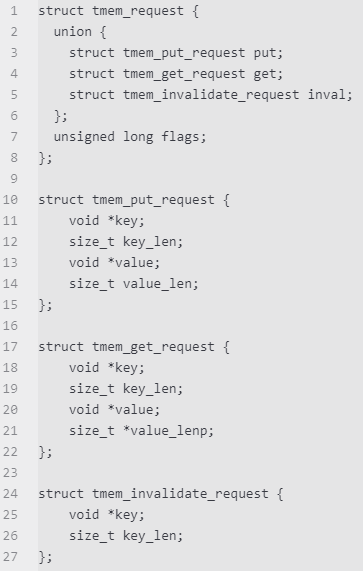
\includegraphics[height=0.4\paperheight]{pictures/struct2.PNG}
  \caption{Το \en{struct tmem\_request } καθώς και δευτερεύοντα
  \en{datatypes} που χρησιμοποιούνται για την μεταφορά δεδομένων}
  \label{fig:structure}
\end{figure}


%syscall
\section{Πρώτη φάση - \en{system call}}

Στο \en{Rumprun} απουσιάζει ο διαχωρισμός των
χώρων χρήστη και χώρο πυρήνα ,
ωστόσο κατά την αρχική υλοποίηση διατηρούμε αυτόν τον , τουλάχιστον
δομικό, διαχωρισμό ώστε η υλοποίηση να μοιάζει περισσότερο με την
αυθεντική υλοποίηση της \en{utmem} σε \en{linux}. Προς αποφυγή
οποιασδήποτε παρεξήγησης,
δεν εννοούμε πως
δημιουργούμε ξεχωριστό χώρο διευθύνσεων, αλλά πως εισάγουμε την
\en{utmem} χαμηλά στην στοίβα λογισμικού, εκεί που παραδοσιακά βρίσκεται
ο χώρο του πυρήνα. Συνεπώς, με βάση αυτήν μας την επιλογή μια «\en{user space}»
εφαρμογή στο \en{Rumprun}, εφόσον
επιθυμεί να χρησιμοποιήσει τις \en{utmem} λειτουργίες, οφείλει να ζητήσει
από τον πυρήνα να εκτελέσει τις λειτουργίες αυτές εκ μέρους της,
θεωρώντας πως δεν έχει την ικανότητα να την επιτελέσει η ίδια στο «\en{user space}».
\newline

Στην αυθεντική υλοποίηση του \en{utmem} μηχανισμού προστέθηκε μια \en{virtual device}
στο λειτουργικό, την οποία οι εφαρμογές χρησιμοποιούσαν μέσω \en{ioctl}
κλήσεις συστήματος. Στην \en{Rumprun} υλοποίηση προσθέσαμε απλά μια
νέα κλήση συστήματος \en{(system call)} του \en{NetBSD} , την οποία ονομάσαμε
\en{tmem} με αριθμό 483, η οποία υποστηρίζει τις τρεις βασικές λειτουργίες
(\en{operations}) της \en{utmem} με βάση το \en{KVM}, δηλαδή \en{Put, Get, Invalidate}.
Αυτή η κλήση συστήματος αντικαθιστά την χρήση της \en{ioctl} από
την εφαρμογή. Εν τέλει, η κλήση συστήματος θα μεταφραστεί
σε κλήση συνάρτησης από τα \en{rump kernels}, όταν δημιουργηθεί το
τελικό \en{unikernel}. Για να γίνει αυτό, φροντίσαμε να ενημερώσουμε
τα \en{rump kernels} για την ύπαρξη αυτής της νέας κλήσης συστήματος, έτσι
ώστε κατά το \en{build} του \en{toolchain} να συμπεριληφθεί , ώστε στην
συνέχεια να είναι διαθέσιμη κατά το \en{bake} των \en{unikernel}.
\newline

Επιλέξαμε την εισαγωγή της νέας κλήσης συστήματος καθώς από πλευράς έκτασης
κώδικα και χρήσης από
μια «\en{user space}» εφαρμογή είναι απλούστερο από το να εισάγουμε
μια εικονική συσκευή όπως στην αυθεντική \en{utmem}. Μην ξεχνάμε
πως βασική φιλοσοφία των \en{unikernels} είναι η ελαχιστοποίηση
του αποτυπώματος των εφαρμογών που εκτελούνται. Άλλωστε, δεν αποτελεί
την τελική μορφή όπως θα φανεί και στην συνέχεια.
\newline

Η ροή των ενεργειών που θα ακολουθηθεί όταν μια
εφαρμογή-\en{unikernel} επιθυμεί να αποθηκεύσει στον \en{host}
ένα κομμάτι της μνήμης του στον \en{guest}, μέσω του \en{operation} \en{Put}, είναι η εξής:
\begin{enumerate}
  \item Η εφαρμογή γεμίζει μια περιοχή μνήμης της με δεδομένα.
  Αυτά τα δεδομένα σκοπεύει να τα δώσει στον \en{host}, ώστε να μπορεί να στη συνέχεια
  να αποδεσμεύσει αυτήν την περιοχή μνήμης.

  \item Εκτελεί την κλήση συστήματος \en{tmem}, όπου δηλώνει
  την διεύθυνση μνήμης της περιοχής, το όνομα του κλειδιου
  με το οποίο θα αναφερόμαστε σε αυτή, και το μέγεθος της. Η
  ροή περνά στο «\en{kernel space}».

  \item O πυρήνας αντιγράφει τα δεδομένα σε δικό του χώρο,
  ελέγχει πως όλα είναι σωστά, και εκτελεί το \en{KVM hypercall}
  που αφορά την \en{tmem} και συγκεκριμένα το \en{Put operation}.

  \item Το \en{backend} λαμβάνει το \en{hypercall request} και
  αναλαμβάνει να αποθηκεύσει την μνήμη που ζητήθηκε. Η
  συμπεριφορά του είναι ίδια με την περίπτωση που
  είχαμε \en{virtualized guest} ως κανονικό λειτουργικό. Το \en{backend}
  δεν είναι σε θέση να γνωρίζει το είδος της εικονικής μηχανής που έστειλε το
  αίτημα.

  \item Εφόσον όλα πήγαν καλά, επιστρέφεται μήνυμα επιτυχίας
  στον \en{guest} μέχρι και το «\en{user space}» επίπεδο. Πλέον η
  εφαρμογή μπορεί να αποδεσμεύσει την μνήμη.

\end{enumerate}

Η ροή για τα \en{Put} και \en{Invalidate operation} είναι αντίστοιχη με τα παραπάνω.
\newline






\subsection{Τεχνικές δυσκολίες}
Όπως ήταν αναμενόμενο, για να υλοποιηθεί το παραπάνω εμφανίστηκαν
μερικές τεχνικές δυσκολίες.
\newline

Η πρώτη τεχνική δυσκολία στην υλοποίηση του μηχανισμού επικοινωνίας με
τον \en{KVM hypervisor}, και άρα και με τις \en{paravirtualization} ευκολίες
που προσφέρει, είναι πως στο \en{NetBSD} δεν υπάρχει έτοιμος μηχανισμός
(\en{API}) ώστε να εκτελούνται \en{hypercalls} με βάση το \en{KVM} ως \en{hypervisor}.
Αντίθετα στο \en{linux} αυτό το \en{task} είναι πιο απλό. Εκεί υπάρχουν έτοιμες
συναρτήσεις του χώρου πυρήνα\cite{KVMhyper},
ονόματι \en{kvm\_hypercall}Χ,  όπου Χ+1 ο αριθμός των \en{argument} που πρέπει να
γνωρίζει ο \en{host} για την εξυπηρέτηση της \en{hypercall}. Ο \en{tmem} μηχανισμός
για \en{hypercall}  χρειάζεται τρια \en{arguments}, τον κωδικό της \en{tmem}, τον
κωδικό του \en{tmem operation}, και το \en{tmem request structure} το οποίο
εκθέτουμε στον \en{host} ως ανταλλακτήριο πληροφοριών.
\newline

Η λύση στο πρόβλημα αυτό είναι να εξάγουμε από το \en{source tree} του \en{linux} τις
απαραίτητες γραμμές και να τις προσθέσουμε στην κλήση συστήματός μας.
Αυτό αυτομάτως περιορίζει την υλοποίησή μας σε αρχιτεκτονική \en{x}86,
η οποία, όμως, είναι η πλέον δημοφιλής και άρα δεν αποτελεί
μεγάλο μειονέκτημα. Ακολουθήσαμε λοιπόν την ροή της \en{kvm\_hypercall2}
στο \en{linux}, και καταλήγουμε σε περίπου 60 γραμμές \en{x}86 \en{assembly}. Το
πιο σημαντικό εντός αυτών είναι πως εκτελείται ένα \en{X86\_FEATURE\_VMMCALL} με
νούμερο (8*32+15) το οποίο όπως αναμενόταν αφορά το \en{KVM hypervisor}
στην \en{x}86 αρχιτεκτονική. Παίρνοντας αυτές τις γραμμές από τον
πηγαίο κώδικα του \en{linux} και τοποθετώντας τες σε ένα \en{header file},
η \en{system call} που υλοποιούμε είναι σε θέση να καλεί \en{KVM hypercalls}
ακόμα και ως \en{Rumprun unikernel}.
\newline

Το επόμενο βήμα είναι να καλέσουμε \en{KVM hypercall} για
χρήση της \en{utmem} συγκεκριμενα. Τα \en{operation codes} και \en{type code} της \en{utmem}
είναι γνωστά από την αυθεντική υλοποίηση και μπορούν να μεταφερθούν αυτούσια.
\newline

Εδώ εμφανίζεται και η δεύτερη τεχνική δυσκολία, η οποία
είναι η έκθεση (\en{expose}) των πληροφοριών μας στον \en{host} που
αναλαμβάνει την εξυπηρέτηση των \en{hypercall} μας. O μηχανισμός
\en{utmem} χρησιμοποιεί \en{instances} του \en{tmem\_request struct} ώστε να
μεταφέρεται η πληροφορία από τον \en{host} στον \en{guest} ή ανάποδα.
Το συγκεκριμένο \en{struct} φέρει την τιμή του ζευγαριού \en{key-value}
καθώς και βοηθητικές πληροφορίες που έχουν να κάνουν με το μέγεθος
της εκάστοτε τιμής. Δυστυχώς ο \en{host} και ο \en{guest} «ζουν» σε
διαφορετικούς χώρους μνήμης (\en{memory space}) και χρειάζεται μετάφραση
σε φυσικό χώρο διευθύνσεων (\en{physical address space}), τον οποίο
ο \en{host} είναι σε θέση να προσπελάσει. Η αυθεντική υλοποίηση της \en{utmem}
μεταφράζει \en{page-aligned virtual addresses} σε \en{physical address}. Η
ευθυγράμμιση σε επίπεδο σελίδας (\en{page alignment}) δεν είναι
απαραίτητη και φαίνεται πως είναι κατάλοιπο από τα αρχικά στάδια
της υλοποίησης του μηχανισμού της \en{utmem}, οπότε επιλέξαμε να την
αγνοήσουμε στην δική μας υλοποίηση. Τονίζουμε πως αυτό δεν επηρεάζει την ορθή
επικοινωνία μεταξύ των δύο πλευρών. Για να επιτύχουμε την μετάφραση από
\en{virtual address} σε \en{physical address} χρησιμοποιούμε την
συνάρτηση \en{vtophys}() που προσφέρει το \en{NetBSD} σε χώρο πυρήνα,
ενώ παράλληλα την υποστηρίζουν και τα \en{rump kernels}.
\newline

Υλοποιήσαμε συνεπώς ό,τι χρειάζεται η \en{system call} μας και
πλέον έχουμε ένα μηχανισμό αντίστοιχο με της αυθεντικής υλοποίησης
της \en{utmem}, ο οποίος μπορεί να χρησιμοποιηθεί σε \en{unikernel}
περιβάλλον. Όλος ο κώδικας δεν ξεπερνά τις 450 γραμμές,
αρκετές από τις οποίες είναι αντίγραφα κώδικα του πυρήνα
του \en{Linux} και δεν έχουν γραφτεί από εμάς.

\begin{figure}[h]
  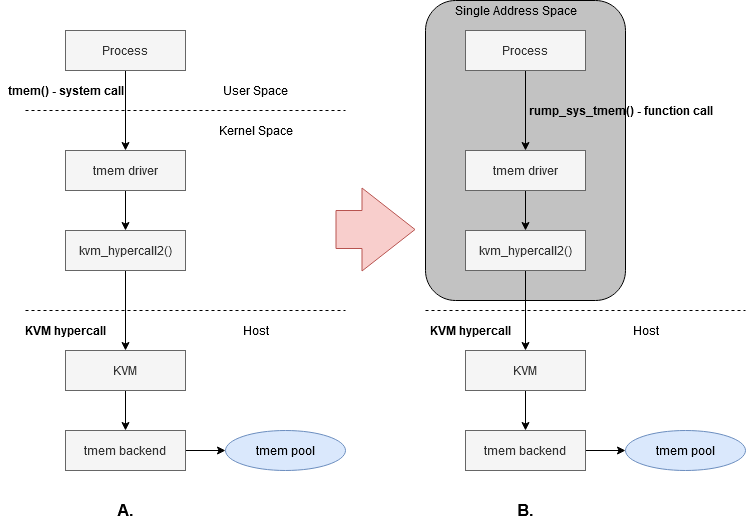
\includegraphics[width=\textwidth]{pictures/syscallFlow.png}
  \caption{Α.Ροή εκτέλεσης της \en{system call tmem()} στο \en{NetBSD}
   Β. H μετατροπή της σε \en{function call} από τα \en{rump kernels}}
  \label{fig:syscallFlow}
\end{figure}




\section{Δεύτερη φάση - \en{function call}}

Όπως αναφέραμε, στο \en{Rumprun} υπάρχει μόνο ένας χώρος διευθύνσεων
καθώς εφαρμογή και πυρήνας γίνονται \en{bake} σε ένα σώμα, το
\en{unikernel}. Ως εκ τούτου, η αρχική μας προσέγγιση διαχωρισμού είναι κενή σημασίας,
απλά βοηθά στην καλύτερη κατανόηση της ροής αφού θυμίζει
περισσότερο παραδοσιακό περιβάλλον. Θα ήταν σαφώς καλύτερο να
εκμεταλλευτούμε την χαρακτηριστική αυτή ιδιότητα ώστε η υλοποίησή μας να
έχει ελάχιστο αποτύπωμα στο περιβάλλον ανάπτυξης.
\newline

Με μια προσεχτική ματία στον κώδικα, η μόνη εξάρτηση από συνάρτηση του πυρήνα,
αντίστοιχη της οποίας δεν υπάρχει σε χώρο χρήστη, είναι για
την μετάφραση από \en{virtual} σε \en{physical addresses} μέσω της
\en{vtophys}(). Η υλοποίηση αυτής στα \en{rump kernels} είναι εξαιρετικά
απλή, το οποίο μας επιτρέπει την αντιγράψουμε
σε «\en{user space}» επίπεδο, δηλαδή στα ανώτερα στρώματα της στοίβας του λογισμικού.
Παίρνουμε λοιπόν ό,τι χρειάζεται και για την εκτέλεση του
\en{hypercall} και πλέον μπορούμε να έχουμε όλη τη λειτουργικότητα
της \en{utmem} δίχως την ανάγκη μιας \en{system call}. Δημιουργήσαμε μια
βιβλιοθήκη, έτοιμη να συμπεριληφθεί στον κώδικα από οποιοδήποτε πρόγραμμα το
επιθυμεί. Ό,τι κάναμε πριν εντός της \en{system call} το κάνουμε τώρα
σε ένα «\en{user space}» \en{.c file}, το οποίο ως σχεδίαση είναι σαφώς
απλούστερο από πριν.
\newline

Από την μια, η ανάπτυξη εφαρμογών γίνεται ελαφρώς πιο σύνθετη, καθώς
πρέπει να προστεθεί κατά το \en{linking} αυτών και ο κώδικας
που εκτελεί τα \en{hypercall} και προσφέρει τα \en{utmem operations},
σε αντίθεση με την \en{system call} όπου η \en{libc} αναλαμβάνει την
αντιστοιχία. Από την άλλη, όμως, το κέρδος είναι πως πλέον δεν απαιτούνται
αλλαγές στο \en{Rumprun-rump kernels}. Η τελική μορφή των δύο εκδώσεων διαφέρει ελάχιστα,
καθώς η \en{system call tmem} της πρώτης φάσης
εν τέλει μεταφράζεται σε ένα απλό \en{function call} από το \en{Rumprun},
με αποτέλεσμα το \en{overhead} να είναι ίδιο στις δύο περιπτώσεις. Μια μικρή διαφορά
είναι πως η function call απαιτεί μια αντιγραφή λιγότερη των δεδομένων.
\newline

Συντονιζόμαστε, συνεπώς, με την φιλοσοφία πίσω από τα \en{rump kernels},
δηλαδή την ανάπτυξη και εκτέλεση \en{drivers} από τον χώρο χρήστη,
δίχως να απαιτείται η προσαρμογή του υφιστάμενου πυρήνα. Ο \en{driver}
μας είναι όλος ο κώδικας που αναλαμβάνει να εκτελέσει την κλήση
επόπτη, και να ανταλλάξει με ασφάλεια τα κομμάτια μνήμη μεταξύ
του \en{guest} και του \en{host}.

\begin{figure}[h]
  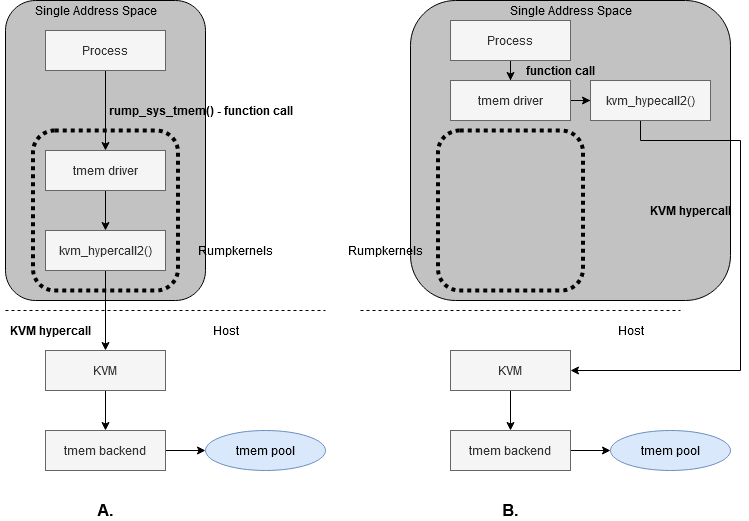
\includegraphics[width=\textwidth]{pictures/sys-func_diff.png}
  \caption{A.\en{Utmem} στο \en{Rumprun} ως \en{system call}
   Β. \en{Utmem} στο \en{Rumprun} ως \en{function call}}
  \label{fig:syscall_funcall}
\end{figure}
